\subsection{ChatterBot Math Calculations}\label{subsec:bot4} 
\begin{figure}[h!tbp]
    \centering
    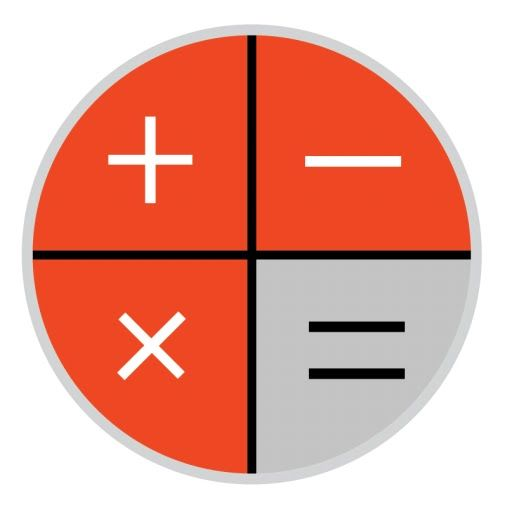
\includegraphics[width=0.1\linewidth]{img/bot4_logo.png}
    \caption{Avatar do perfil do Math Calculations.}
    \label{fig:bot4_logo}
\end{figure}

A proposta do Chatterbot Math é oferecer um bot de calculadora no chat do aplicativo Kik\footnote{O Kik é uma apicação de mensagens instantâneas, vide \url{www.kik.com}} que está disponível pra os sistemas operacional Android e iOS. Para acessá-lo basta procurar o nome dele no buscador do aplicativo. Esse chatterbot foi implementado na linguagem Python e somente em Inglês.

O início da interação com ele se deu da seguinte forma:
\begin{description}
    \item \eu{hi}
    \item \chatbot{I don't think that was an expression for me to solve! Or ty changing your formatting.}
    \item Clicando na única opção do menu: \eu{Help!}
    \item \chatbot{
Hello! I'm the calculator bot, you can send me things to calculate. Here are a few examples: \\ \\
'1+1'
'9*38(139.192/123,3)' \\ \\
And so on... it's also possible to type like a normal person like: \\ \\
'1 plus 1' \\
'9 times 38 (129.192 divided by 123,3)' \\
'square root of 4' \\
Or even 'hello tell me what is 1 multiplied by 12983.32 divided by 9 \\ \\
So you can replace
+ with 'plus', \\
- with 'minus' \\
/ with 'divided by', \\
* with 'times' or 'x' or 'multiplied by', \\
\textasciicircum with 'to the power of', \\
root with 'square root' and 
\% with 'mod' \\
The bot also has the following functions: sin, cos, tan, asin, acos, atan, log \\
Example: 'sin 45 plus log 19 - (8 \textasciicircum sin 45)' \\ \\
Goodluck!}
\end{description}
\begin{figure}[h!tbp]
    \centering
    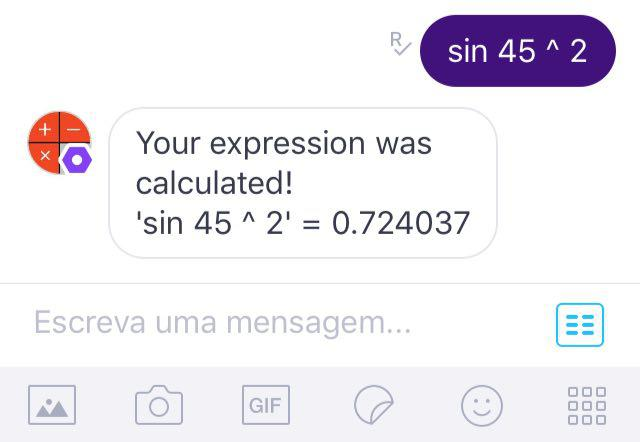
\includegraphics[width=0.4\linewidth]{img/bot4_1.png}
    % \caption{Screenshot da resposta do Math Calculations.}
    \label{fig:bot4_1}
\end{figure}

Após um período de testes, percebi que esse bot não suporta o cálculo do fatorial. Apesar disso, ao enviar a mensagem ``100!'', o bot não informou que ele desconhecia o perador ``!'', apenas o ignorou.
Essa falha, nos permite obter $11$ como resultado da mensagem $10! + 1$. Porém, como o chatterbot retorna mensagens no formato \textsc{expressão = resultado}, facilmente percebemos que o fatorial não foi utilizado.